\documentclass[../the.tex]{subfiles}


\begin{document}


\section{Tổng quan về tách phông ảnh}
\label{tong_quan}
{\fontsize{13}{12} \selectfont
Hiện nay, các tập đoàn công nghệ không ngừng đầu tư và ứng dụng các loại công nghệ trong đó có tách phông ảnh vào các sản phẩm công ty của họ đem lại doanh thu cũng như thu hút lượng khách hàng rất lớn, mang lại trải nghiệm mới mẻ cho người dùng. Cụ thể, tập đoàn Bkav thay vì tốn chi phí cho phần cứng phải đầu tư máy ảnh kép, họ tiết kiệm chi phí bằng cách tích hợp khả năng tách phông vào máy chụp ảnh trên điện thoại cho phép người dùng làm mờ cảnh xung quanh người, làm nổi bật đối tượng được chụp. Ứng dụng SNOW \cite{snow} ra đời cho phép ghép ảnh, thêm các chi tiết như râu, nón, mắt kiếng,... lên từng bộ phận đã được tách phông trên mặt người trực tiếp khi quay rất độc đáo. Ngoài ra, phải kể đến thành công của tách phông ảnh khi làm nổi bật các bộ phận trong cơ thể con người như tim, gan, phổi,... từ ảnh X-quang hoặc tách phông thiết bị máy móc y học khi hoạt động phẫu thuật trong cơ thể người.}
\bigskip

{\fontsize{13}{12} \selectfont
Tách phông ảnh là quá trình cho phép tạo ra những hình ảnh mới từ ảnh gốc với những vùng chi tiết quan trọng được giữ lại, xóa bỏ những vùng nền không có tác dụng phục vụ rất nhiều cho y tế, phần mềm công nghệ máy ảnh, đồ họa kỹ thuật số và tất nhiên chúng đòi hỏi thách thức cao khi thực hiện. Với những lợi ích đem lại cũng cho thấy tính cần thiết của vai trò tách phông ảnh cần được nghiên cứu, đầu tư nhiều hơn. Tách phông ảnh thực sự là ứng dụng của bài toán phân vùng ngữ nghĩa đối tượng người trong ảnh, chúng giải quyết vấn đề xác định vị trí chính xác của đối tượng chiếm trong ảnh, khắc phục nhược điểm của bài toán phát hiện đối tượng khi chỉ có khả năng xác định khung chứa đại khái đối tượng.}  
\bigskip
 

{\fontsize{13}{12} \selectfont
\begin{figure}[H]
\centering
\tikzset{every picture/.style={line width=0.75pt}} %set default line width to 0.75pt        

\begin{tikzpicture}[x=0.75pt,y=0.75pt,yscale=-1,xscale=1]
%uncomment if require: \path (0,300); %set diagram left start at 0, and has height of 300

%Image [id:dp5541696886497023] 
\draw (155.25,139.5) node  {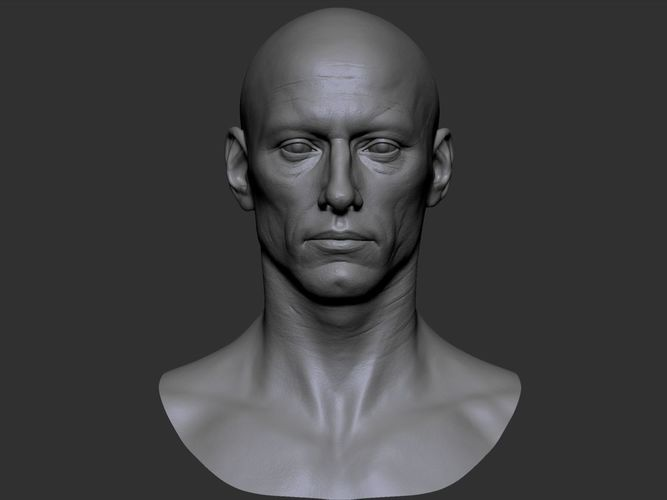
\includegraphics[width=130pt,height=110pt]{face.jpg}};
%Image [id:dp6999670900516217] 
\draw (504.25,139.5) node  {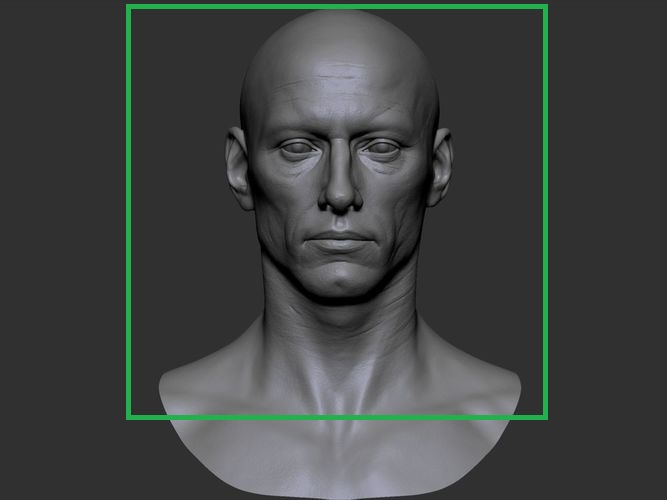
\includegraphics[width=130pt,height=110pt]{cnn.jpg}};
%Right Arrow [id:dp363270476880974] 
\draw  [fill={rgb, 255:red, 0; green, 255; blue, 73 }  ,fill opacity=1 ] (299,138) -- (341,138) -- (341,128) -- (369,148) -- (341,168) -- (341,158) -- (299,158) -- cycle ;

\end{tikzpicture}
	\caption{Phát hiện đối tượng thông thường (Nguồn: www.cgtrader.com)}
	\label{fig:detect}
\end{figure}}

\bigskip




\end{document}